%%%%%%%%%%%%%%%%%%%%%%%%%%%%%%%%%%%%%%%%%%%%%%%%%%%%%%%%%%
%  Projektdokumentation Web-Engineering II - SoSe2026
%  Gruppe2 - Projekt A (GuardX) + Projekt B (SunShine Tours)
%
%  Basiert auf dem DHBW-Mannheim-LaTeX-Template
%  (Drabant / Pfisterer / Reichwald), schlank angepasst
%  fuer eine Projektdokumentation.
%
%  Kompilieren:  pdflatex master  ->  biber master  ->
%                pdflatex master  ->  pdflatex master
%  (oder einfach:  latexmk -pdf master)
%%%%%%%%%%%%%%%%%%%%%%%%%%%%%%%%%%%%%%%%%%%%%%%%%%%%%%%%%%

\documentclass[fontsize=12pt,BCOR=5mm,DIV=15,parskip=half,listof=totoc,
               paper=a4,toc=bibliography,pointlessnumbers]{scrreprt}

%% Sprache & Kodierung
\usepackage[utf8]{inputenc}
\usepackage[T1]{fontenc}
\usepackage[ngerman]{babel}
\usepackage[german=quotes]{csquotes}

%% Literatur (biblatex + biber)
\usepackage[backend=biber, autocite=inline, style=numeric]{biblatex}
\addbibresource{bibliography.bib}
\DefineBibliographyStrings{ngerman}{andothers = {{et\,al\adddot}},}

%% Grafik, Tabellen, Code
\usepackage{graphicx}
\usepackage{xcolor}
\usepackage{listings}
\usepackage{array}
\usepackage{tabularx}
\usepackage{longtable}
\usepackage{booktabs}
\usepackage{caption}
\usepackage[german]{varioref}
\usepackage[nohyperlinks]{acronym}
\usepackage{setspace}
\usepackage{tocloft}
\usepackage{fnpct}
\usepackage{calc}
\usepackage[hidelinks=true]{hyperref}

%% Schriftfamilie ohne Serifen (wie im DHBW-Template)
\renewcommand*{\familydefault}{\sfdefault}
\addtokomafont{disposition}{\sffamily}
\addtokomafont{chapter}{\Large}
\addtokomafont{section}{\large}
\addtokomafont{subsection}{\normalsize}
\addtokomafont{part}{\LARGE}
\setlength{\emergencystretch}{3em}

%% Tabellen lesbarer: linksbuendiger Flattersatz statt Blocksatz,
%% etwas mehr Zeilenhoehe. \newcolumntype{L} = ragged-right p-Spalte.
\newcolumntype{L}[1]{>{\raggedright\arraybackslash}p{#1}}
\renewcommand{\tabularxcolumn}[1]{>{\raggedright\arraybackslash}p{#1}}
\renewcommand{\arraystretch}{1.18}

%%%%%%%%%%%%%%%%%%%%%%%%%%%%%%%%%%%%%%%%%%%%%%%%%%%%%%%%%%
%  Kopf- und Fusszeile
%%%%%%%%%%%%%%%%%%%%%%%%%%%%%%%%%%%%%%%%%%%%%%%%%%%%%%%%%%
\RequirePackage[automark]{scrlayer-scrpage}
\renewcommand{\chaptermarkformat}{}
\RedeclareSectionCommand[beforeskip=0pt]{chapter}
\clearpairofpagestyles
\ofoot[\rule{0pt}{\ht\strutbox+\dp\strutbox}\pagemark]{\rule{0pt}{\ht\strutbox+\dp\strutbox}\pagemark}
\ohead{\headmark}

%% Part-Titel oben auf der Seite statt vertikal zentriert,
%% damit das nachfolgende Kapitel auf derselben Seite beginnen kann.
\renewcommand*\partheadstartvskip{\vspace*{2\baselineskip}}
\renewcommand*\partheadendvskip{\vskip 2\baselineskip}

%%%%%%%%%%%%%%%%%%%%%%%%%%%%%%%%%%%%%%%%%%%%%%%%%%%%%%%%%%
%  Metadaten
%%%%%%%%%%%%%%%%%%%%%%%%%%%%%%%%%%%%%%%%%%%%%%%%%%%%%%%%%%
\newcommand{\imagedir}{img}
% Rot markierte Platzhalter, die das Team noch ausfuellen sollte:
\newcommand{\platzhalter}[1]{\textcolor{red}{[#1]}}

% Platzhalterbox fuer noch einzufuegende Screenshots
\newcommand{\screenshot}[1]{%
  \fbox{\begin{minipage}[c][4.2cm][c]{0.82\textwidth}%
  \centering\itshape\color{gray} Platzhalter f\"ur Screenshot:\\[2mm] #1%
  \end{minipage}}%
}

\hypersetup{pdftitle={GuardX und SunShine Tours - Projektdokumentation},
            pdfauthor={Gruppe2}}

%% Titelseiten-Angaben
\newcommand{\DieArtDerArbeit}{Projektdokumentation}
\newcommand{\DerTitelDerArbeit}{GuardX \& SunShine Tours}
\newcommand{\DerUntertitel}{Dokumentation der Web-Engineering-II-Projekte A und B}
\newcommand{\DieKursbezeichnung}{MA-TINF25CS2}
\newcommand{\DerStudiengang}{Informatik - Cyber Security}
\newcommand{\DerWissBetreuer}{Dipl.-Ing.\ Udo Erdmann}
\newcommand{\DerStudiengangsleiter}{\platzhalter{Name Studiengangsleiter}}
\newcommand{\DerBearbeitungszeitraum}{Sommersemester 2026}
\newcommand{\DasAbgabedatum}{30.06.2026}

%%%%%%%%%%%%%%%%%%%%%%%%%%%%%%%%%%%%%%%%%%%%%%%%%%%%%%%%%%
%  Listings-Stil (PHP / JS / SQL)
%%%%%%%%%%%%%%%%%%%%%%%%%%%%%%%%%%%%%%%%%%%%%%%%%%%%%%%%%%
\renewcommand{\lstlistingname}{Quelltext}
\renewcommand{\lstlistlistingname}{Quelltextverzeichnis}

\definecolor{codebg}{rgb}{0.97,0.97,0.97}
\definecolor{codekw}{rgb}{0.13,0.29,0.53}
\definecolor{codecomment}{rgb}{0.30,0.55,0.30}
\definecolor{codestring}{rgb}{0.64,0.08,0.08}
\definecolor{codenum}{rgb}{0.5,0.5,0.5}

\lstdefinestyle{projektstil}{
    backgroundcolor=\color{codebg},
    basicstyle=\ttfamily\footnotesize,
    keywordstyle=\color{codekw}\bfseries,
    commentstyle=\color{codecomment}\itshape,
    stringstyle=\color{codestring},
    numberstyle=\tiny\color{codenum},
    numbers=left,
    numbersep=8pt,
    captionpos=b,
    breaklines=true,
    showstringspaces=false,
    frame=single,
    rulecolor=\color{gray!40},
    tabsize=2,
    columns=fullflexible,
    upquote=true,
    extendedchars=true,
    literate={ä}{{\"a}}1 {ö}{{\"o}}1 {ü}{{\"u}}1
             {Ä}{{\"A}}1 {Ö}{{\"O}}1 {Ü}{{\"U}}1
             {ß}{{\ss}}1
}
\lstset{style=projektstil}

%%%%%%%%%%%%%%%%%%%%%%%%%%%%%%%%%%%%%%%%%%%%%%%%%%%%%%%%%%

\begin{document}

%%% Titelseite
% !TEX root = master.tex
\begin{titlepage}
\begin{center}


\includegraphics[width=0.45\textwidth]{\imagedir/logo.jpg}\\[3em]

{\textsf{\large Duale Hochschule Baden-W\"urttemberg Mannheim}}\\[3em]

{\textsf{\textbf{\large \DieArtDerArbeit}}}\\[8mm]

{\textsf{\textbf{\Huge \DerTitelDerArbeit}}}\\[5mm]

{\textsf{\large \DerUntertitel}}\\[2cm]

{\textsf{\textbf{\large Studiengang \DerStudiengang}}}\\[1mm]
{\textsf{Kurs \DieKursbezeichnung}}

\vfill

\begin{minipage}{0.9\textwidth}
\renewcommand{\arraystretch}{1.4}
\begin{tabbing}
\hspace{5cm}\=\kill
\textbf{Team:} \> Gruppe2 \\[2mm]
\textbf{Teammitglieder:} \> Moritz Brenner \hfill \\
 \> Maik Baumg\"artner \hfill \\
 \> Marcel Reinholz \hfill \\
 \> Jakob Goelden \hfill \\[2mm]
\textbf{Wiss. Betreuer:} \> \DerWissBetreuer \\[1mm]
\textbf{Abgabedatum:} \> \DasAbgabedatum
\end{tabbing}
\end{minipage}

\end{center}
\end{titlepage}

\pagenumbering{roman}
\normalfont

%%% Verzeichnisse
\tableofcontents
\cleardoublepage

\phantomsection
\addcontentsline{toc}{chapter}{\listfigurename}
\listoffigures
\enlargethispage{3\baselineskip}
\begingroup
  \let\clearpage\relax
  \let\cleardoublepage\relax
  \vspace{0.5\baselineskip}
  \phantomsection
  \addcontentsline{toc}{chapter}{\listtablename}
  \listoftables
  \vspace{0.5\baselineskip}
  \lstlistoflistings
  \vspace{0.5\baselineskip}
  % !TEX root = master.tex
\chapter*{Abk\"urzungsverzeichnis}
\addcontentsline{toc}{chapter}{Abk\"urzungsverzeichnis}

\begin{acronym}[XAMPP]
\acro{agb}[AGB]{Allgemeine Gesch\"aftsbedingungen}
\acro{ajax}[AJAX]{Asynchronous JavaScript and XML}
\acro{api}[API]{Application Programming Interface}
\acro{cidr}[CIDR]{Classless Inter-Domain Routing}
\acro{crud}[CRUD]{Create, Read, Update, Delete}
\acro{csrf}[CSRF]{Cross-Site Request Forgery}
\acro{css}[CSS]{Cascading Style Sheets}
\acro{dom}[DOM]{Document Object Model}
\acro{exif}[EXIF]{Exchangeable Image File Format}
\acro{html}[HTML]{Hypertext Markup Language}
\acro{http}[HTTP]{Hypertext Transfer Protocol}
\acro{json}[JSON]{JavaScript Object Notation}
\acro{php}[PHP]{PHP: Hypertext Preprocessor}
\acro{sql}[SQL]{Structured Query Language}
\acro{xampp}[XAMPP]{Cross-Platform, Apache, MariaDB, PHP, Perl}
\acro{xss}[XSS]{Cross-Site Scripting}
\end{acronym}

\endgroup
\cleardoublepage

\onehalfspacing

%%% Beginn Fliesstext
\clearpage
\ihead{\chaptername~\thechapter}
\pagenumbering{arabic}

% !TEX root = master.tex
\chapter{Einleitung}
\label{ch:einleitung}

Diese Dokumentation fasst die beiden im Rahmen der Vorlesung \emph{Web-/App-Engineering~II}
(Kurs \DieKursbezeichnung, Sommersemester~2026) von \textbf{Gruppe2} entwickelten Projekte zusammen.
Beide Projekte wurden als Teamarbeit umgesetzt; die Dokumentation ist bewusst als \emph{ein}
gemeinsames Dokument angelegt und in zwei Teile gegliedert.

\textbf{Teil~I} beschreibt das Projekt~A \emph{GuardX} -- eine datenbankgest\"utzte Web-App mit
Session- und Benutzerverwaltung, Admin-Bereich und mehreren sicherheitsorientierten Werkzeugen.
\textbf{Teil~II} beschreibt das Projekt~B \emph{SunShine~Tours} -- eine responsive Web-Seite f\"ur
ein (fiktives) St\"adte-Tour-Unternehmen mit Echtzeit-Kostenberechnung und dateibasierter
Buchungsverwaltung. W\"ahrend Projekt~A den Schwerpunkt auf Sicherheit, Sessions und
Datenbankzugriffe legt, steht bei Projekt~B die clientseitige Interaktivit\"at sowie die
KI-gest\"utzte Erstellung s\"amtlicher Inhalte und Grafiken im Vordergrund.

\section{Zielsetzung der Dokumentation}
Ziel dieser Dokumentation ist es, beide Anwendungen so zu beschreiben, dass sie auf einem
fremden System nachvollziehbar installiert, gestartet und bewertet werden k\"onnen. Daf\"ur werden
je Projekt die Funktionalit\"at, der Aufbau des Frontends, die Verzeichnis- und ggf.
Datenstruktur sowie alle ben\"otigten Zugangsdaten dargestellt. Besonderer Wert wird auf die
Nachvollziehbarkeit gelegt: F\"ur jede geforderte Funktionalit\"at wird in einer
Zuordnungstabelle angegeben, in welchem Skript sie umgesetzt ist (vgl.
Kapitel~\ref{ch:a-funktionen} bzw.~\ref{ch:b-funktionen}).

\section{Aufbau des Dokuments}
Nach dieser Einleitung gliedert sich das Dokument wie folgt. Teil~I (Projekt~A) beginnt mit einem
Referenzdokument (Ziele, Funktionsrahmen, Projektrahmen, Umsetzungsstrategie sowie Aufgaben und
Zust\"andigkeiten), gefolgt vom Product-Backlog, der Beschreibung von Frontend, Verzeichnisstruktur
und Datenbank, der funktionalen Umsetzung sowie einer Installationsanleitung inklusive Zugangsdaten.
Teil~II (Projekt~B) beschreibt analog \"Uberblick und Umfang, die eingesetzten KI-Systeme und
Werkzeuge, die funktionale Umsetzung, die Verzeichnisstruktur und die Installation. Den Abschluss
bildet ein kurzes Fazit.


%%%%%%%%%%%%%%%%%%%%%%%%%%%%%%%%%%%%%%%%%%%%%%%%%%%%%%%%%%
%  TEIL I  -  PROJEKT A: GuardX
%%%%%%%%%%%%%%%%%%%%%%%%%%%%%%%%%%%%%%%%%%%%%%%%%%%%%%%%%%
\part{Projekt A: GuardX}
\let\svdclearpage\clearpage
\let\svdcleardoublepage\cleardoublepage
\let\clearpage\relax
\let\cleardoublepage\relax
% !TEX root = master.tex
\chapter{Referenzdokument}
\label{ch:a-referenz}

\section{Ziele}
\emph{GuardX} ist ein modulares \enquote{Web Security \& Privacy Toolkit}. Ziel des Projekts ist
eine Web-App, die registrierten Nutzerinnen und Nutzern mehrere praxisnahe Werkzeuge rund um
digitale Sicherheit und Privatsph\"are an einer Stelle bereitstellt und dabei selbst nach
g\"angigen Sicherheitsprinzipien aufgebaut ist. Die App verfolgt damit einen doppelten Zweck:
Zum einen liefert sie konkreten Nutzen (Passw\"orter pr\"ufen, Bild-Metadaten entfernen,
Tracking-Risiken verstehen), zum anderen demonstriert sie die im Modul geforderten technischen
Konzepte -- insbesondere Sessionverwaltung, sichere Authentifizierung, Rechteverwaltung und
Datenbankzugriffe.

\section{Funktionsrahmen}
Die Anwendung gliedert sich in einen \textbf{Account- und Verwaltungsbereich} und drei
\textbf{Fachmodule}.

Der Account- und Verwaltungsbereich umfasst:
\begin{itemize}
  \item Registrierung, Login und Logout mit serverseitiger Validierung,
  \item Sessionverwaltung mit automatischem Logout nach konfigurierbarer Inaktivit\"at,
  \item einen Admin-Bereich mit vollst\"andiger Benutzerverwaltung (\ac{crud}),
  \item Passwortverwaltung (\"Andern durch Nutzer, Zur\"ucksetzen durch Admin) und
  \item eine Rechteverwaltung mit den Rollen \emph{Admin} und \emph{User}.
\end{itemize}

Die drei Fachmodule sind:
\begin{itemize}
  \item \textbf{Metadaten-Bereiniger}: Entfernt \ac{exif}-Daten aus hochgeladenen Bildern und
        bietet die ausgelesenen Metadaten als \ac{json}-Datei zum Download an.
  \item \textbf{Browser-Fingerprinting}: Macht sichtbar, welche Merkmale (Canvas, WebGL,
        Zeitzone, Sprache, Hardware) einen Browser identifizierbar machen.
  \item \textbf{Live-Passwort-Checker}: Pr\"uft per \ac{ajax} in Echtzeit die Passwortst\"arke und
        gleicht das Passwort datenschutzfreundlich (k-Anonymity) gegen bekannte Datenlecks ab.
\end{itemize}

Querschnittlich werden die geforderten Technologien eingesetzt: client- und serverseitige
Eingabepr\"ufung (u.\,a. mit regul\"aren Ausdr\"ucken), Einbindung von jQuery/jQuery~UI und
Bootstrap, dynamisches Nachladen via \ac{ajax}, Meldungs- und Best\"atigungsdialoge, Datenexport
via \ac{json} sowie eine dynamische, responsive Men\"ustruktur. Eine vollst\"andige Zuordnung
dieser Funktionen zu den jeweiligen Skripten findet sich in Kapitel~\ref{ch:a-funktionen}.

\section{Projektrahmen}
Das Projekt wurde als zeitlich begrenzte Teamarbeit von vier Personen im Sommersemester~2026
umgesetzt. Die technologischen Rahmenbedingungen entsprechen den Projektvorgaben:

\begin{table}[htbp]
\centering
\caption{Technologischer Rahmen von Projekt~A}
\label{tab:a-rahmen}
\begin{tabularx}{\textwidth}{@{}lX@{}}
\toprule
\textbf{Bereich} & \textbf{Technologie} \\
\midrule
Client       & HTML5, \ac{css}, JavaScript; jQuery, jQuery~UI, Bootstrap~5.3 \\
Server       & Apache, \ac{php}~8.2.4 (ohne Framework) \\
Datenbank    & MariaDB~10.4.28 \\
Laufzeitumgebung & XAMPP \\
Versionsverwaltung & Git / GitHub \\
\bottomrule
\end{tabularx}
\end{table}

Auf den Einsatz fertiger Frameworks (z.\,B. Angular, Vue, Symfony, React) wurde vorgabengem\"a\ss{}
verzichtet; eingesetzt werden ausschlie\ss{}lich die erlaubten Bibliotheken jQuery, jQuery~UI und
Bootstrap.

\section{Umsetzungsstrategie}
Die Entwicklung erfolgte iterativ und arbeitsteilig. Zur Zusammenarbeit wurde ein
Git-Feature-Branch-Workflow genutzt: Neue Funktionen wurden in eigenen Branches entwickelt,
per Pull-Request zusammengef\"uhrt und vor dem Merge daraufhin gepr\"uft, ob die Anwendung unter
XAMPP lauff\"ahig bleibt. Wiederkehrende Bestandteile (Header/Navigation, Footer, Konfiguration)
wurden als wiederverwendbare Includes ausgelagert, sodass alle Seiten ein einheitliches
Erscheinungsbild und Verhalten besitzen. Sicherheitsrelevante Mechanismen
(\ac{csrf}-Schutz, Passwort-Hashing, Prepared Statements) wurden von Beginn an mitgedacht und
sind zentral umgesetzt. Vor der Abgabe wurde die Installierbarkeit auf einem frischen System
getestet.

\section{Aufgaben und Zust\"andigkeiten}
Die Arbeitspakete wurden wie in Tabelle~\ref{tab:a-zustaendig} dargestellt verteilt. Die
Zuordnung orientiert sich an den jeweils verantworteten Komponenten; \"ubergreifende Aufgaben
(Code-Reviews, Integration, Test) wurden gemeinsam wahrgenommen.

\begin{table}[htbp]
\centering
\caption{Aufgaben und Zust\"andigkeiten in Projekt~A}
\label{tab:a-zustaendig}
\begin{tabularx}{\textwidth}{@{}lX@{}}
\toprule
\textbf{Teammitglied} & \textbf{Verantwortungsbereich} \\
\midrule
Maik Baumg\"artner & Backend: Session- und Benutzerverwaltung, Login/Logout/Registrierung,
  Admin-Bereich, Datenbankanbindung und -schema, zentrale Hilfsfunktionen sowie
  Navigations-Templates. \\
\addlinespace
Marcel Reinholz & Footer und alle dar\"uber verlinkten Rechtsseiten (Impressum, Datenschutz,
  AGB) sowie das Modul der API-Aufrufe (Live-Passwort-Checker, Leak-Abgleich). \\
\addlinespace
Jakob Goelden & Modul Browser-Fingerprinting (\texttt{info.php}) sowie Einrichtung und
  Pflege des GitHub-Repositories (Branch-/Merge-Strategie, Versionsverwaltung). \\
\addlinespace
Moritz Brenner & Modul Metadaten-Bereiniger, das durchg\"angige \ac{css}-Design
  (Layout, Cyber-Theme, responsive Anpassungen) sowie die Startseite. \\
\bottomrule
\end{tabularx}
\end{table}

\let\clearpage\svdclearpage
\let\cleardoublepage\svdcleardoublepage
% !TEX root = master.tex
\chapter{Product-Backlog}
\label{ch:a-backlog}

Das Product-Backlog wurde \"uber die gesamte Projektlaufzeit gepflegt und priorisiert. Es
bildet die umgesetzten Anforderungen ab und ordnet jeder Anforderung eine Priorit\"at, eine
Aufwandssch\"atzung in Story~Points (SP), die verantwortliche Person sowie den Bearbeitungsstatus
zu. Zum Abgabezeitpunkt sind alle Eintr\"age umgesetzt. Tabelle~\ref{tab:a-backlog} zeigt das
vollst\"andige Backlog.

\begin{small}
\begin{longtable}{@{}L{0.95cm} L{6.9cm} L{1.1cm} L{0.7cm} L{1.7cm} L{1.6cm}@{}}
\caption{Product-Backlog Projekt~A (GuardX)}
\label{tab:a-backlog}\\
\toprule
\textbf{Nr.} & \textbf{Anforderung} & \textbf{Prio} & \textbf{SP} & \textbf{Zust\"andig} & \textbf{Status} \\
\midrule
\endfirsthead
\multicolumn{6}{c}{\tablename~\thetable{} -- Fortsetzung}\\
\toprule
\textbf{Nr.} & \textbf{Anforderung} & \textbf{Prio} & \textbf{SP} & \textbf{Zust\"andig} & \textbf{Status} \\
\midrule
\endhead
\midrule
\multicolumn{6}{r}{\footnotesize Fortsetzung n\"achste Seite}\\
\endfoot
\bottomrule
\endlastfoot

A-01 & Sessionverwaltung inkl.\ CSRF-Token-Erzeugung & Hoch & 5 & Maik & Erledigt \\
A-02 & Registrierung mit serverseitiger Pr\"ufung und Passwort-Hashing & Hoch & 5 & Maik & Erledigt \\
A-03 & Login/Logout mit Rollenweiterleitung (Admin/User) & Hoch & 5 & Maik & Erledigt \\
A-04 & Automatisches Logout nach konfigurierbarer Inaktivit\"at & Hoch & 3 & Maik & Erledigt \\
A-05 & CSRF-Schutz f\"ur alle schreibenden Formulare & Hoch & 3 & Maik & Erledigt \\
A-06 & Brute-Force-Schutz: Login-Sperre nach Fehlversuchen & Mittel & 3 & Maik & Erledigt \\
A-07 & Rate-Limiting der Registrierung pro IP-Adresse & Mittel & 3 & Marcel & Erledigt \\
A-08 & Admin: Benutzer anlegen und l\"oschen & Hoch & 5 & Maik & Erledigt \\
A-09 & Admin: Rolle umschalten, E-Mail und Passwort setzen & Hoch & 5 & Maik & Erledigt \\
A-10 & Rechteverwaltung: Zugriffsschutz f\"ur Admin-Seiten & Hoch & 3 & Maik & Erledigt \\
A-11 & Self-Service: E-Mail/Passwort \"andern, Account l\"oschen & Mittel & 5 & Maik & Erledigt \\
A-12 & Zentrale Konfiguration \"uber Konfigurationsdatei & Mittel & 2 & Maik & Erledigt \\
A-13 & Dynamische, responsive Navigation (Desktop/Mobile) & Hoch & 5 & Maik & Erledigt \\
A-14 & Session-Timeout-Warndialog mit jQuery~UI & Mittel & 3 & Maik & Erledigt \\
A-15 & Modul Metadaten-Bereiniger: EXIF-Daten entfernen & Hoch & 8 & Moritz & Erledigt \\
A-16 & Ausgelesene EXIF-Daten als JSON-Export anbieten & Mittel & 3 & Moritz & Erledigt \\
A-17 & Automatische Bildrotation anhand EXIF-Orientierung & Niedrig & 3 & Moritz & Erledigt \\
A-18 & Modul Browser-Fingerprinting (Canvas, WebGL, u.\,a.) & Hoch & 8 & Jakob & Erledigt \\
A-19 & Modul Live-Passwort-Checker (AJAX, Regex-St\"arke) & Hoch & 8 & Marcel & Erledigt \\
A-20 & Leak-Abgleich via HaveIBeenPwned (k-Anonymity) & Mittel & 5 & Marcel & Erledigt \\
A-21 & Rechtsseiten Impressum/Datenschutz/AGB inkl.\ Footer & Mittel & 3 & Marcel & Erledigt \\
A-22 & Durchg\"angiges CSS-Design (Cyber-Theme, responsive) & Mittel & 8 & Moritz & Erledigt \\
A-23 & Sichere IP-Ermittlung hinter Proxy/Cloudflare & Niedrig & 3 & Maik & Erledigt \\
A-24 & Git-Repository, Branch- und Merge-Workflow & Mittel & 3 & Jakob & Erledigt \\
A-25 & Abgabevorbereitung (SQL-Dump, php.ini-Hinweise, Test) & Hoch & 3 & Alle & Erledigt \\
\end{longtable}
\end{small}

% !TEX root = master.tex
\chapter{Aufbau und Bedienbarkeit (Frontend)}
\label{ch:a-frontend}

Das Frontend von GuardX folgt durchg\"angig der klassischen Struktur aus Kopfbereich mit
Navigation, Inhaltsbereich und Footer. Gestalterisch kommt ein dunkles \enquote{Cyber-Theme}
mit gr\"unen Akzenten zum Einsatz, das auf allen Seiten \"uber eine gemeinsame Stylesheet-Basis
(\texttt{style/main.css}, \texttt{style/navbar.css}) erzeugt wird.

\section{Navigation}
Die Navigation ist sowohl \emph{dynamisch} als auch \emph{responsiv} umgesetzt. Serverseitig
wird in jedem Seitenaufruf \"uber die Funktion \texttt{is\_mobile()} anhand des User-Agents
entschieden, ob die Desktop-Navigation (\texttt{template/navbar.php}) oder die mobile Variante
mit Hamburger-Men\"u (\texttt{template/navbar\_mobile.php}) eingebunden wird. Die angezeigten
Men\"upunkte h\"angen zus\"atzlich vom Login-Status und der Rolle ab: Nicht angemeldete Nutzer
sehen einen \emph{Login}-Punkt, angemeldete Nutzer den Bereich \emph{Mein Bereich} und
Administratoren zus\"atzlich \emph{System Admin}. Die Links werden \"uber die Hilfsfunktion
\texttt{get\_url()} erzeugt, damit sie unabh\"angig vom Installationsverzeichnis korrekt
aufl\"osen.

\begin{figure}[htbp]
    \centering
    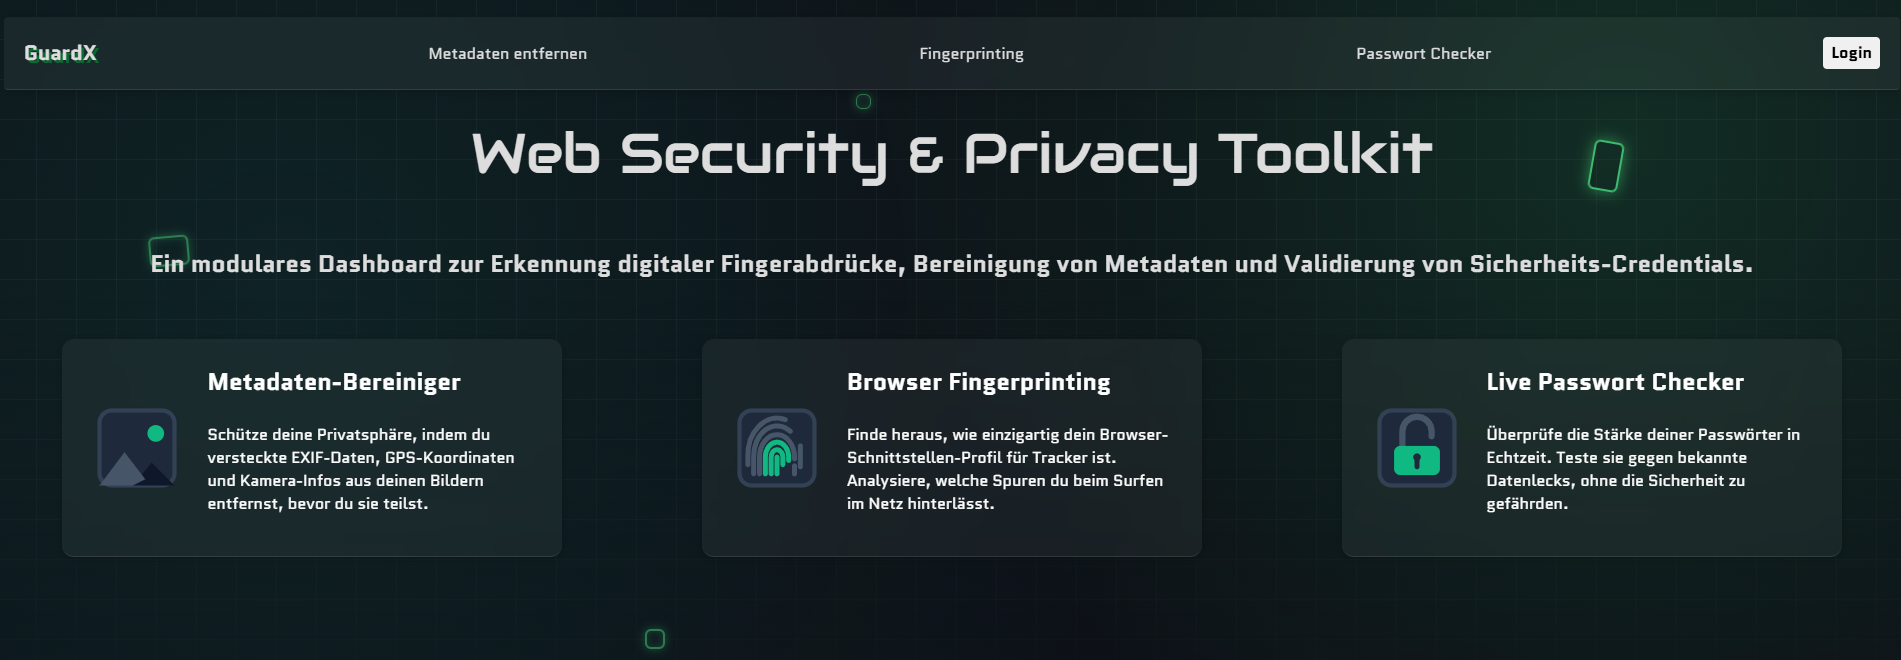
\includegraphics[width=0.8\textwidth]{img/navigation.png}
    \caption{Startseite (Dashboard) mit Desktop-Navigation und den drei Modulkacheln}
    \label{fig:a-start}
\end{figure}

\section{Startseite}
Die Startseite (\texttt{index.php}) dient als Dashboard und stellt die drei Fachmodule als
Kacheln mit kurzer Beschreibung vor: Metadaten-Bereiniger, Browser-Fingerprinting und
Live-Passwort-Checker. Von hier aus gelangt man per Klick direkt in das jeweilige Modul.

\section{Registrierung, Login und gesch\"utzte Bereiche}
\"Uber \texttt{auth.php} erfolgen Registrierung und Login in einem gemeinsamen, umschaltbaren
Formular. Nach erfolgreichem Login wird der Nutzer rollenabh\"angig weitergeleitet -- als Admin
in das Admin-Dashboard, sonst in den pers\"onlichen Bereich. R\"uckmeldungen (Erfolg, Fehler,
Sperrhinweise) werden direkt am Formular angezeigt.

Der \textbf{pers\"onliche Bereich} (\texttt{user.php}) erlaubt das \"Andern der E-Mail-Adresse
und des Passworts (mit Best\"atigung des aktuellen Passworts) sowie das L\"oschen des eigenen
Accounts. Sicherheitskritische Aktionen werden \"uber einen Best\"atigungsdialog abgesichert.

Der \textbf{Admin-Bereich} (\texttt{admin.php}) bietet eine tabellarische Benutzer\"ubersicht
mit Inline-Formularen, \"uber die Administratoren neue Benutzer anlegen, E-Mail-Adressen und
Passw\"orter setzen, die Rolle umschalten und Benutzer l\"oschen k\"onnen. Der eigene Account ist
gegen versehentliches L\"oschen gesch\"utzt.

\begin{figure}[htbp]
\centering
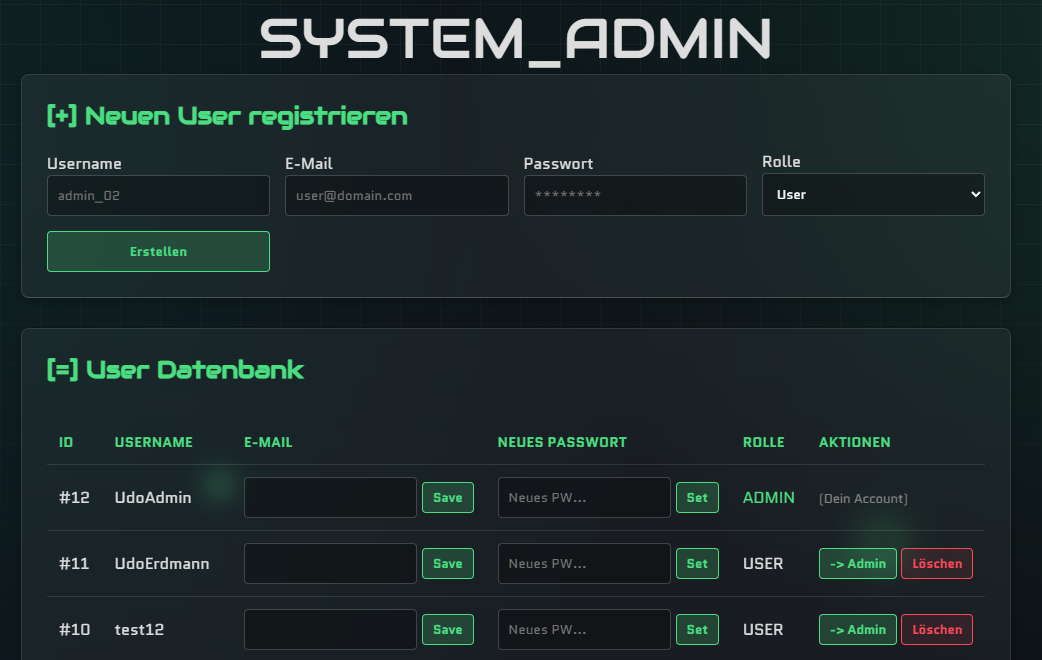
\includegraphics[width=0.8\textwidth]{img/admin-dashboard.png}
\caption{Admin-Bereich mit Benutzerverwaltung}
\label{fig:a-admin}
\end{figure}

\section{Fachmodule}
\textbf{Metadaten-Bereiniger.} \"Uber ein Upload-Formular wird ein Bild hochgeladen; die
Anwendung liest die \ac{exif}-Daten aus, bietet sie als \ac{json}-Datei zum Download an und
liefert eine von Metadaten bereinigte Kopie des Bildes zur\"uck. Das Original wird nach der
Verarbeitung serverseitig gel\"oscht.

\textbf{Browser-Fingerprinting.} Die Seite (\texttt{info.php}) stellt anschaulich dar, welche
Merkmale einen Browser identifizierbar machen (u.\,a. Canvas- und WebGL-Fingerprint, Zeitzone,
Sprache, Hardware). Die Werte werden clientseitig per JavaScript ermittelt und hervorgehoben.

\textbf{Live-Passwort-Checker.} Bei jeder Eingabe wird das Passwort per \ac{ajax} an den Server
geschickt und sofort bewertet: Die Anforderungen an die St\"arke (L\"ange, Gro\ss-/Kleinbuchstaben,
Ziffern, Sonderzeichen) werden mit regul\"aren Ausdr\"ucken gepr\"uft, zus\"atzlich erfolgt ein
datenschutzfreundlicher Abgleich gegen bekannte Datenlecks. Ein Auge-Symbol blendet das Passwort
bei Bedarf ein.

\section{Meldungen und Dialoge}
F\"ur Hinweise und Best\"atigungen werden zwei Mechanismen verwendet: einfache
\texttt{confirm()}-Dialoge f\"ur destruktive Aktionen (z.\,B. Benutzer l\"oschen) sowie ein
modaler jQuery-UI-Dialog, der vor Ablauf der Session erscheint und die Wahl zwischen
\emph{Bleiben} und \emph{Ausloggen} bietet.

% !TEX root = master.tex
\chapter{Verzeichnisstruktur (Backend / Webserver)}
\label{ch:a-verzeichnis}

Das Projektverzeichnis wird vollst\"andig in das Webserver-Wurzelverzeichnis (bei XAMPP
\texttt{htdocs}) installiert. Alle internen Pfade sind relativ aufgel\"ost, sodass das Projekt
unabh\"angig vom Ordnernamen lauff\"ahig ist. Die folgende \"Ubersicht zeigt die Struktur:

\begin{lstlisting}[numbers=none]
guardx/
|-- index.php                 Startseite / Dashboard
|-- init.php                  Session-Start, Timeout, CSRF-Token
|-- config.php                Zentrale Konfiguration (DB-Verbindung)
|-- functions.php             Server-Hilfsfunktionen (IP, Pfade, Mobile)
|-- functions.js              Client-Logik (Session-Timer, Menue)
|-- auth.php                  Login / Registrierung / Logout
|-- user.php                  Persoenlicher Bereich (Profil)
|-- admin.php                 Admin-Bereich (Benutzerverwaltung, CRUD)
|-- admin_logout.php          Logout-Endpunkt
|-- keep_alive.php            Session am Leben halten (AJAX-Ziel)
|-- impressum.php             Impressum
|-- datenschutz.php           Datenschutzerklaerung
|-- agb.php                   AGB
|-- php.ini.hinweise          Hinweise zu benoetigten PHP-Extensions
|
|-- db/
|   |-- users.sql             Aktueller DB-Dump (Struktur + Daten)
|   |-- init_databases.sql    Aelterer Dump (siehe Hinweis Kap. 8)
|
|-- include/
|   |-- api-calls/
|   |   |-- skript.php         Oberflaeche Live-Passwort-Checker
|   |   |-- check.php          AJAX-Endpunkt: Staerke + Leak-Abgleich
|   |-- fingerprinting/
|   |   |-- info.php           Modul Browser-Fingerprinting
|   |-- metadata_stripping/
|       |-- metadata_stripping.php  Modul Metadaten-Bereiniger
|       |-- uploads/           (zur Laufzeit erzeugt) Upload-Ablage
|       |-- clean/             (zur Laufzeit erzeugt) bereinigte Bilder + JSON
|
|-- template/
|   |-- navbar.php             Desktop-Navigation
|   |-- navbar_mobile.php      Mobile Navigation (Hamburger)
|   |-- footer.php             Footer mit Rechts-Links
|
|-- style/
    |-- main.css               Basis-/Layout-Styles (Cyber-Theme)
    |-- navbar.css             Navigationsstyles
    |-- metadata_stripping.css Styles des Metadaten-Moduls
\end{lstlisting}

\noindent Die Verzeichnisse \texttt{include/metadata\_stripping/uploads/} und
\texttt{.../clean/} werden vom Modul bei Bedarf automatisch angelegt; sie m\"ussen f\"ur den
Webserver-Benutzer beschreibbar sein. Tabelle~\ref{tab:a-verzeichnis} fasst die Aufgaben der
wichtigsten Komponenten zusammen.

\begin{small}
\begin{longtable}{@{}L{4.4cm} L{9.9cm}@{}}
\caption{Komponenten von Projekt~A}
\label{tab:a-verzeichnis}\\
\toprule
\textbf{Datei / Verzeichnis} & \textbf{Aufgabe} \\
\midrule
\endfirsthead
\toprule
\textbf{Datei / Verzeichnis} & \textbf{Aufgabe} \\
\midrule
\endhead
\bottomrule
\endfoot
\bottomrule
\endlastfoot
\texttt{init.php} & Startet/erneuert die Session, erzwingt das Inaktivit\"ats-Timeout und erzeugt das CSRF-Token. Wird von praktisch allen Seiten eingebunden. \\
\texttt{config.php} & Zentrale Konfigurationsdatei mit den Verbindungsdaten zur Datenbank; wird per \texttt{require\_once} eingebunden. \\
\texttt{functions.php} & Serverseitige Hilfsfunktionen: sichere IP-Ermittlung, Pfad-Helfer (\texttt{get\_url}), Mobile-Erkennung (\texttt{is\_mobile}). \\
\texttt{functions.js} & Clientseitige Logik: Session-Timer mit jQuery-UI-Dialog, mobiles Men\"u, Login-Weiterleitung. \\
\texttt{auth.php} & Registrierung, Login und Logout inkl.\ Validierung, Hashing, Brute-Force- und Rate-Limit-Schutz. \\
\texttt{user.php} & Pers\"onlicher Bereich: E-Mail/Passwort \"andern, Account l\"oschen. \\
\texttt{admin.php} & Admin-Bereich mit vollst\"andiger Benutzerverwaltung (Anlegen, \"Andern, Rolle, L\"oschen). \\
\texttt{include/api-calls/} & Live-Passwort-Checker: Oberfl\"ache (\texttt{skript.php}) und AJAX-Endpunkt (\texttt{check.php}). \\
\texttt{include/fingerprinting/} & Modul Browser-Fingerprinting (\texttt{info.php}). \\
\texttt{metadata\_stripping/} & Modul Metadaten-Bereiniger inkl.\ Lauf\-zeit-Ordnern f\"ur Upload und bereinigte Ausgabe. \\
\texttt{template/} & Wiederverwendbare Bausteine: Desktop-/Mobil-Navigation und Footer. \\
\texttt{style/} & Stylesheets f\"ur Layout, Navigation und Metadaten-Modul. \\
\texttt{db/} & SQL-Dumps der Datenbank (Struktur und Daten). \\
\bottomrule
\end{longtable}
\end{small}

% !TEX root = master.tex
\chapter{Datenstrukturen und Tabellen (SQL-Server)}
\label{ch:a-datenbank}

Die Anwendung nutzt die MariaDB-Datenbank \texttt{users}. Sie umfasst drei Tabellen: \texttt{user}
f\"ur die Benutzerkonten sowie \texttt{login\_logs} und \texttt{register\_logs} f\"ur
sicherheitsrelevante Protokollierung. Alle Tabellen besitzen einen aufsteigenden
Prim\"arschl\"ussel \texttt{id}. Zwischen \texttt{login\_logs.user\_id} und \texttt{user.id}
besteht eine logische Zuordnung (Fremdschl\"usselbeziehung), die in der Anwendung ausgewertet wird.

\section{Tabelle \texttt{user}}
Speichert die Benutzerkonten. Das Passwort wird ausschlie\ss{}lich als bcrypt-Hash abgelegt;
\texttt{is\_admin} steuert die Rolle.

\begin{table}[htbp]
\centering
\caption{Spalten der Tabelle \texttt{user}}
\label{tab:db-user}
\begin{tabularx}{\textwidth}{@{}l l X@{}}
\toprule
\textbf{Spalte} & \textbf{Typ} & \textbf{Bedeutung} \\
\midrule
\texttt{id}       & INT, PK, AUTO\_INCREMENT & Eindeutige Benutzer-ID \\
\texttt{username} & TEXT, NOT NULL           & Anmeldename (eindeutig gepr\"uft) \\
\texttt{email}    & VARCHAR(100), NULL       & Optionale E-Mail-Adresse \\
\texttt{password} & VARCHAR(255), NOT NULL   & bcrypt-Hash des Passworts \\
\texttt{is\_admin}& TINYINT(1), Default 0    & Rolle: 1 = Admin, 0 = User \\
\texttt{zeit}     & DATE, Default heute      & Anlagedatum des Kontos \\
\bottomrule
\end{tabularx}
\end{table}

\begin{lstlisting}[language=SQL,caption={CREATE-Statement der Tabelle \texttt{user}},label={lst:db-user}]
CREATE TABLE `user` (
  `id`       int(11)      NOT NULL,
  `username` text         NOT NULL,
  `email`    varchar(100) DEFAULT NULL,
  `password` varchar(255) NOT NULL,
  `is_admin` tinyint(1)   NOT NULL DEFAULT 0,
  `zeit`     date         NOT NULL DEFAULT current_timestamp()
) ENGINE=InnoDB DEFAULT CHARSET=latin1 COLLATE=latin1_swedish_ci;
\end{lstlisting}

\section{Tabelle \texttt{login\_logs}}
Protokolliert jeden Login-Versuch. Anhand der fehlgeschlagenen Versuche eines Nutzers innerhalb
eines Zeitfensters wird die Brute-Force-Sperre umgesetzt.

\begin{table}[htbp]
\centering
\caption{Spalten der Tabelle \texttt{login\_logs}}
\label{tab:db-loginlogs}
\begin{tabularx}{\textwidth}{@{}l l X@{}}
\toprule
\textbf{Spalte} & \textbf{Typ} & \textbf{Bedeutung} \\
\midrule
\texttt{id}         & INT, PK, AUTO\_INCREMENT & Eindeutige Log-ID \\
\texttt{user\_id}   & INT, NOT NULL            & Bezug auf \texttt{user.id} \\
\texttt{ip\_address}& VARCHAR(45)              & IP-Adresse (IPv4/IPv6) \\
\texttt{login\_time}& DATETIME, Default jetzt  & Zeitpunkt des Versuchs \\
\texttt{success}    & TINYINT(1), Default 1    & 1 = erfolgreich, 0 = fehlgeschlagen \\
\bottomrule
\end{tabularx}
\end{table}

\section{Tabelle \texttt{register\_logs}}
Protokolliert Registrierungen je IP-Adresse und erm\"oglicht so das Rate-Limiting (maximale Anzahl
neuer Konten pro IP und Tag).

\begin{table}[htbp]
\centering
\caption{Spalten der Tabelle \texttt{register\_logs}}
\label{tab:db-registerlogs}
\begin{tabularx}{\textwidth}{@{}l l X@{}}
\toprule
\textbf{Spalte} & \textbf{Typ} & \textbf{Bedeutung} \\
\midrule
\texttt{id}           & INT, PK, AUTO\_INCREMENT & Eindeutige Log-ID \\
\texttt{ip\_address}  & VARCHAR(45)              & IP-Adresse der Registrierung \\
\texttt{attempt\_time}& DATETIME, Default jetzt  & Zeitpunkt der Registrierung \\
\bottomrule
\end{tabularx}
\end{table}

Alle Datenbankzugriffe erfolgen ausschlie\ss{}lich \"uber \emph{Prepared Statements}, um
SQL-Injection zu verhindern~\autocite{php-preparedstatements}. Die vollst\"andige Struktur
inklusive Beispieldaten liegt im Dump \texttt{db/users.sql} (vgl.\ Kapitel~\ref{ch:a-installation}).

% !TEX root = master.tex
\chapter{Funktionale Umsetzung: Funktion und Skript}
\label{ch:a-funktionen}

Dieses Kapitel ordnet jede geforderte Funktionalit\"at dem Skript bzw.\ der Datei zu, in der sie
umgesetzt ist. Damit ist nachvollziehbar, wo eine bestimmte Funktion zu finden ist
(vgl.\ Abgabevorgabe zur Nachvollziehbarkeit). Tabelle~\ref{tab:a-funktionen} gibt die
vollst\"andige Zuordnung an.

\begingroup
\small
\setlength{\tabcolsep}{5pt}
\renewcommand{\arraystretch}{1.3}
\begin{longtable}{@{}L{4.2cm} L{4.6cm} L{4.7cm}@{}}
\caption{Zuordnung Funktionalit\"at zu Skript (Projekt~A)}
\label{tab:a-funktionen}\\
\toprule
\textbf{Funktionalit\"at} & \textbf{Skript / Datei} & \textbf{Kurzbeschreibung} \\
\midrule
\endfirsthead
\multicolumn{3}{@{}l}{\small\itshape Tabelle \thetable{} -- Fortsetzung}\\
\midrule
\textbf{Funktionalit\"at} & \textbf{Skript / Datei} & \textbf{Kurzbeschreibung} \\
\midrule
\endhead
\midrule
\multicolumn{3}{r@{}}{\footnotesize\itshape Fortsetzung n\"achste Seite}\\
\endfoot
\bottomrule
\endlastfoot

\multicolumn{3}{@{}l}{\textbf{Account, Session und Rechteverwaltung}}\\*
\addlinespace[0.4ex]
Sessionverwaltung & \texttt{init.php} & Session-Start und -Wiederherstellung, CSRF-Token \\
Login / Logout & \texttt{auth.php}, \texttt{admin\_logout.php} & Anmeldung, Rollenweiterleitung, Abmeldung \\
Registrierung & \texttt{auth.php} & Serverseitige Pr\"ufung neuer Konten \\
Automatisches Logout & \texttt{init.php}, \texttt{functions.js} & Timeout-Pr\"ufung (Server) und Warndialog (Client) \\
Benutzerverwaltung (CRUD) & \texttt{admin.php} & Anlegen, \"Andern, Rolle, L\"oschen \\
Rechteverwaltung (Rollen) & \texttt{init.php}, \texttt{admin.php} & Zugriffsschutz \"uber \texttt{is\_admin} \\
Self-Service-Profil & \texttt{user.php} & E-Mail/Passwort \"andern, Account l\"oschen \\
Zentrale Konfiguration & \texttt{config.php} & DB-Zugangsdaten, per \texttt{require\_once} \\
\addlinespace[0.8ex]

\multicolumn{3}{@{}l}{\textbf{Sicherheit}}\\*
\addlinespace[0.4ex]
CSRF-Schutz & \texttt{init.php} (+ Pr\"ufung in \texttt{admin.php}, \texttt{user.php}, \texttt{auth.php}) & Token-Erzeugung und -Pr\"ufung je Formular \\
Passwort-Hashing & \texttt{auth.php} & bcrypt via \texttt{password\_hash}/\texttt{verify} \\
Brute-Force-Schutz & \texttt{auth.php}, Tabelle \texttt{login\_logs} & Sperre nach mehreren Fehlversuchen \\
Rate-Limiting (Registrierung) & \texttt{auth.php}, Tabelle \texttt{register\_logs} & Begrenzung neuer Konten pro IP \\
Prepared Statements & \texttt{auth.php}, \texttt{admin.php}, \texttt{user.php} & Schutz vor SQL-Injection \\
Eingabevalidierung (RegExp) & \texttt{functions.js}, \texttt{check.php}, \texttt{auth.php} & Client- und serverseitig, regul\"are Ausdr\"ucke \\
\addlinespace[0.8ex]

\multicolumn{3}{@{}l}{\textbf{Oberfl\"ache, Bibliotheken und AJAX}}\\*
\addlinespace[0.4ex]
jQuery / jQuery~UI & \texttt{functions.js} & Timeout-Dialog, DOM-Interaktion \\
Bootstrap-Einbindung & \texttt{template/}, \texttt{style/} & Layout- und Komponentenraster \\
AJAX-Nachladen & \texttt{api-calls/check.php}, \texttt{keep\_alive.php} & Live-Pr\"ufung, Session-Verl\"angerung \\
Meldungs-/Best\"atigungsdialoge & \texttt{functions.js}, \texttt{template/footer.php} & \texttt{confirm()} und jQuery-UI-Dialog \\
Dynamische, responsive Navigation & \texttt{template/navbar.php}, \texttt{navbar\_mobile.php} & rollenabh\"angig, \texttt{is\_mobile()}, \texttt{get\_url()} \\
\addlinespace[0.8ex]

\multicolumn{3}{@{}l}{\textbf{Fachmodule und weitere Seiten}}\\*
\addlinespace[0.4ex]
JSON-Datenexport & \texttt{metadata\_stripping.php} & EXIF-Daten als JSON-Download \\
Datei-Upload & \texttt{metadata\_stripping.php} & Bild-Upload und -Bereinigung \\
Externer API-Aufruf & \texttt{api-calls/check.php} & Leak-Abgleich (HaveIBeenPwned) \\
Browser-Fingerprinting & \texttt{fingerprinting/info.php} & Canvas, WebGL, Zeitzone u.\,a. \\
Rechtsseiten & \texttt{impressum.php}, \texttt{datenschutz.php}, \texttt{agb.php} & \"uber den Footer verlinkt \\
\end{longtable}
\endgroup

\section{Sicherheitsmechanismen im Detail}
Die sicherheitsrelevanten Funktionen sind bewusst zentral umgesetzt:

\textbf{CSRF-Schutz.} F\"ur jede Session wird in \texttt{init.php} ein Zufalls-Token erzeugt. Jedes
schreibende Formular f\"uhrt das Token mit; serverseitig wird es zeitkonstant gepr\"uft, bevor eine
Aktion ausgef\"uhrt wird~\autocite{owasp-csrf}.

\begin{lstlisting}[language=PHP,caption={Zeitkonstante CSRF-Pr\"ufung (Auszug \texttt{admin.php})},label={lst:a-csrf}]
if (!hash_equals($_SESSION['csrf_token'], $_POST['csrf_token'])) {
    die("CSRF Token ungültig!");
}
\end{lstlisting}

\textbf{Passwort-Hashing.} Passw\"orter werden nie im Klartext gespeichert, sondern mit dem
bcrypt-Verfahren \"uber \texttt{password\_hash()} gehasht und beim Login mit
\texttt{password\_verify()} gepr\"uft~\autocite{php-passwordhash}.

\textbf{Prepared Statements.} S\"amtliche Datenbankabfragen verwenden parametrisierte Abfragen,
sodass Benutzereingaben nicht als SQL interpretiert werden k\"onnen.

\textbf{Brute-Force- und Rate-Limiting.} Fehlgeschlagene Logins werden in \texttt{login\_logs}
protokolliert und f\"uhren nach mehreren Versuchen zu einer tempor\"aren Sperre; Registrierungen
werden \"uber \texttt{register\_logs} je IP begrenzt.

\textbf{Datenschutzfreundlicher Leak-Abgleich.} Beim Passwort-Check wird nur ein Pr\"afix des
SHA-1-Hashes an die externe API gesendet (k-Anonymity); der Abgleich der vollst\"andigen Hashes
erfolgt lokal~\autocite{hibp-range}.

% !TEX root = master.tex
\chapter{Installation und Zugangsdaten}
\label{ch:a-installation}

\section{Systemvoraussetzungen}
GuardX setzt eine Standard-XAMPP-Umgebung voraus: Apache als Webserver, \ac{php}~8.2 sowie
MariaDB. Zus\"atzlich m\"ussen einige PHP-Erweiterungen aktiv sein (siehe unten).

\section{Installationsschritte}
\begin{enumerate}
  \item \textbf{Projekt kopieren.} Den gesamten Projektordner in das Webserver-Wurzelverzeichnis
        legen (bei XAMPP: \texttt{C:\textbackslash\allowbreak xampp\textbackslash\allowbreak htdocs}).
  \item \textbf{PHP-Erweiterungen aktivieren.} In der \texttt{php.ini} (bei XAMPP
        \texttt{C:\textbackslash\allowbreak xampp\textbackslash\allowbreak php\textbackslash\allowbreak php.ini}) m\"ussen die
        Erweiterungen \texttt{gd}, \texttt{mbstring}, \texttt{exif} und \texttt{curl} aktiv (nicht
        auskommentiert) sein. Anschlie\ss{}end Apache neu starten. Die ben\"otigten Eintr\"age sind
        in der mitgelieferten Datei \texttt{php.ini.hinweise} dokumentiert.
  \item \textbf{Datenbank importieren.} In phpMyAdmin eine Datenbank \texttt{users} anlegen und den
        Dump \texttt{db/users.sql} importieren. Damit werden Struktur \emph{und} Beispieldaten
        angelegt.
  \item \textbf{Schreibrechte pr\"ufen.} Die Verzeichnisse unter
        \texttt{include/metadata\_stripping/} (\texttt{uploads/}, \texttt{clean/}) m\"ussen f\"ur
        den Webserver beschreibbar sein. Sie werden bei Bedarf automatisch angelegt.
  \item \textbf{Aufruf.} Die Anwendung \"uber \texttt{http://localhost/\allowbreak<Projektordner>/\allowbreak index.php}
        im Browser \"offnen.
\end{enumerate}

\enlargethispage{4\baselineskip}
\section{Zugangsdaten}
Tabelle~\ref{tab:a-zugang} listet alle f\"ur Betrieb und Bewertung notwendigen Zugangsdaten.

\begin{table}[!ht]
\centering
\caption{Zugangsdaten Projekt~A}
\label{tab:a-zugang}
\begin{tabularx}{\textwidth}{@{}l l X@{}}
\toprule
\textbf{Zweck} & \textbf{Benutzer} & \textbf{Passwort / Wert} \\
\midrule
Datenbank (MariaDB) & \texttt{root} & (leer -- XAMPP-Standard) \\
Datenbankname       & \multicolumn{2}{l}{\texttt{users} (Host: \texttt{localhost})} \\
Demo-Login (User)   & \texttt{UdoErdmann} & \texttt{AbgabeGruppe2} \\
Demo-Login (Admin)  & \texttt{UdoAdmin}   & \texttt{AbgabeGruppe2} \\
\bottomrule
\end{tabularx}
\end{table}

%%%%%%%%%%%%%%%%%%%%%%%%%%%%%%%%%%%%%%%%%%%%%%%%%%%%%%%%%%
%  TEIL II -  PROJEKT B: SunShine Tours
%%%%%%%%%%%%%%%%%%%%%%%%%%%%%%%%%%%%%%%%%%%%%%%%%%%%%%%%%%
\part{Projekt B: SunShine Tours}
\let\svdclearpage\clearpage
\let\svdcleardoublepage\cleardoublepage
\let\clearpage\relax
\let\cleardoublepage\relax
% !TEX root = master.tex
\chapter{\"Uberblick und Umfang}
\label{ch:b-ueberblick}

\emph{SunShine~Tours} ist eine als Demonstrationsprojekt umgesetzte Web-Seite f\"ur einen
fiktiven Anbieter von St\"adtereisen. Die inhaltliche Ausgestaltung ist bewusst satirisch
gehalten; technisch handelt es sich um eine serverseitig mit \ac{php} erzeugte Web-Anwendung,
die ohne Datenbank auskommt und ihre Daten dateibasiert (im \ac{json}-Format) ablegt.

\section{Seiten\"ubersicht}
Die Anwendung besteht aus mehreren Inhaltsseiten mit gemeinsamem Kopf- und Fu\ss{}bereich:
\begin{itemize}
  \item \textbf{Startseite} (\texttt{index.php}) -- Einstieg mit Hero-Bereich und Kennzahlen.
  \item \textbf{\"Uber uns} (\texttt{about.php}) -- Vorstellung des (fiktiven) Teams und der
        Unternehmenswerte.
  \item \textbf{Touren / Kundenstimmen} (\texttt{tours.php}) -- Tour\-angebote und mehrere
        Kundenbewertungen.
  \item \textbf{Buchung} (\texttt{booking.php}) -- Buchungsformular mit Echtzeit-Kostenanzeige.
  \item \textbf{Best\"atigung} (\texttt{confirmation.php}) -- Zusammenfassung nach erfolgreicher
        Buchung.
  \item \textbf{Rechtliches} (\texttt{legal.php}) -- Impressum, Datenschutz und AGB.
  \item \textbf{Formular-Test} (\texttt{formcheck.php}) -- kleine Seite zur Demonstration der
        GET-/POST-Verarbeitung.
\end{itemize}

\section{Gestaltung und technischer Umfang}
Das Layout folgt der Struktur Kopfbereich--Inhalt--Fu\ss{}bereich und ist responsiv umgesetzt.
Die Farbgebung (Gelb-, Orange- und Gr\"unt\"one) ist \"uber \ac{css}-Variablen zentral definiert,
wodurch sich auch ein Hell-/Dunkel-Modus realisieren l\"asst. Das Logo ist vollst\"andig in
\ac{css} gestaltet (ohne Bilddatei). Die auf den Seiten verwendeten St\"adtebilder wurden mit
einem KI-Bildgenerator erzeugt (vgl.\ Kapitel~\ref{ch:b-kitools}).

Der technische Umfang umfasst sieben PHP-Seiten, zwei gemeinsame Includes (Kopf- und
Fu\ss{}bereich), zwei JavaScript-Dateien (Buchungslogik und allgemeine Oberfl\"achenfunktionen)
sowie ein zentrales Stylesheet. Eine Datenbank wird nicht ben\"otigt; Buchungen werden als
\ac{json}-Dateien gespeichert.

% !TEX root = master.tex
\vspace{2\baselineskip}
\chapter{Verwendete KI-Systeme und Werkzeuge}
\label{ch:b-kitools}

Bei der Erstellung von Projekt~B wurden KI-Systeme als unterst\"utzende Werkzeuge eingesetzt.
Die Offenlegung erfolgt gem\"a\ss{} den Projektvorgaben. Tabelle~\ref{tab:b-kitools} fasst die
eingesetzten KI-Systeme und ihren jeweiligen Einsatzzweck zusammen.

\begin{table}[htbp]
\centering
\caption{Eingesetzte KI-Systeme in Projekt~B}
\label{tab:b-kitools}
\begin{tabularx}{\textwidth}{@{}l l X@{}}
\toprule
\textbf{KI-System} & \textbf{Anbieter} & \textbf{Einsatzzweck} \\
\midrule
Claude & Anthropic & Haupts\"achlich genutzt zur Erstellung des Quelltexts (PHP, JavaScript, \ac{css}) sowie der textlichen Inhalte. \\
\addlinespace
Gemini & Google & Erstellung der verwendeten Bilder bzw.\ Grafiken (St\"adtebilder). \\
\bottomrule
\end{tabularx}
\end{table}

Der weit \"uberwiegende Teil des Quelltexts und der Inhalte wurde mit Claude erstellt und
anschlie\ss{}end vom Team gepr\"uft, angepasst und integriert. Die auf den Seiten eingebundenen
St\"adtebilder (\texttt{images/}) wurden mit Gemini generiert.

\section{Weitere Werkzeuge}
Neben den KI-Systemen kamen die folgenden Werkzeuge zum Einsatz: XAMPP als lokale
Laufzeitumgebung (Apache, \ac{php}), Git bzw.\ GitHub zur Versionsverwaltung sowie ein
Webbrowser zum Testen der Anwendung.

\let\clearpage\svdclearpage
\let\cleardoublepage\svdcleardoublepage
% !TEX root = master.tex
\chapter{Funktionale Umsetzung: Funktion und Skript}
\label{ch:b-funktionen}

Analog zu Projekt~A ordnet dieses Kapitel die Funktionalit\"aten den jeweiligen Skripten zu
(Tabelle~\ref{tab:b-funktionen}).

\begingroup
\small
\setlength{\tabcolsep}{5pt}
\renewcommand{\arraystretch}{1.3}
\begin{longtable}{@{}L{4.4cm} L{4.4cm} L{4.7cm}@{}}
\caption{Zuordnung Funktionalit\"at zu Skript (Projekt~B)}
\label{tab:b-funktionen}\\
\toprule
\textbf{Funktionalit\"at} & \textbf{Skript / Datei} & \textbf{Kurzbeschreibung} \\
\midrule
\endfirsthead
\multicolumn{3}{@{}l}{\small\itshape Tabelle \thetable{} -- Fortsetzung}\\
\midrule
\textbf{Funktionalit\"at} & \textbf{Skript / Datei} & \textbf{Kurzbeschreibung} \\
\midrule
\endhead
\midrule
\multicolumn{3}{r@{}}{\footnotesize\itshape Fortsetzung n\"achste Seite}\\
\endfoot
\bottomrule
\endlastfoot

\multicolumn{3}{@{}l}{\textbf{Buchung}}\\*
\addlinespace[0.4ex]
Buchungsformular & \texttt{booking.php} & Eingabemaske f\"ur die Buchung \\
Echtzeit-Kostenberechnung & \texttt{js/booking.js} & Personen $\times$ Tage $\times$ Preis + Ausfl\"uge \\
Dynamische Personenfelder & \texttt{js/booking.js} & Felder je nach Personenzahl \\
Clientseitige Validierung & \texttt{js/booking.js} & Pflichtfelder und Datumspr\"ufung \\
Buchungsverarbeitung & \texttt{process\_booking.php} & POST auswerten, Preis berechnen, Kartennummer maskieren \\
Datenspeicherung (JSON + Zeitstempel) & \texttt{process\_booking.php} & Ablage je Buchung unter \texttt{bookings/} \\
Buchungsbest\"atigung & \texttt{confirmation.php} & Zusammenfassung aus der Session \\
GET-/POST-Demonstration & \texttt{formcheck.php} & Test der Formular\"ubertragung \\
\addlinespace[0.8ex]

\multicolumn{3}{@{}l}{\textbf{Oberfl\"ache und Navigation}}\\*
\addlinespace[0.4ex]
Hell-/Dunkel-Modus & \texttt{js/main.js} & Umschaltung, gespeichert im \texttt{localStorage} \\
Mobiles Men\"u / Navigation & \texttt{js/main.js}, \texttt{includes/header.php} & responsive Navigation \\
News-Ticker / Besucherz\"ahler & \texttt{includes/footer.php} & Z\"ahlung \"uber \texttt{visitor\_count.txt} \\
Gemeinsamer Kopf-/Fu\ss{}bereich & \texttt{includes/header.php}, \texttt{includes/footer.php} & wiederverwendbare Bausteine \\
Gestaltung / Theme & \texttt{css/style.css} & Farbschema, Layout, Hell-/Dunkel-Modus \\
\addlinespace[0.8ex]

\multicolumn{3}{@{}l}{\textbf{Inhaltsseiten}}\\*
\addlinespace[0.4ex]
Kundenstimmen & \texttt{tours.php} & mehrere Bewertungen \\
Teamseite & \texttt{about.php} & Vorstellung des fiktiven Teams \\
Rechtliche Seiten & \texttt{legal.php} & Impressum, Datenschutz, AGB \\
\end{longtable}
\endgroup

\section{Echtzeit-Kostenberechnung}
Die Buchungsseite berechnet den Gesamtpreis ohne Neuladen der Seite. Bei jeder \"Anderung der
Eingaben (Personenzahl, Reisedauer, ausgew\"ahlte Ausfl\"uge) wird der Preis neu ermittelt und als
Zusammenfassung angezeigt. Die Grundkosten ergeben sich aus Personenzahl, Anzahl der Tage und dem
Tagespreis; hinzu kommen die Kosten der gew\"ahlten Ausfl\"uge.

\begin{lstlisting}[language=Java,caption={Kern der Kostenberechnung (Auszug \texttt{js/booking.js})},label={lst:b-cost}]
var baseCost = persons * days * pricePerDay;     // Grundpreis
var excursionCost = 0;                           // Summe der Ausfluege
// ... Aufsummieren der ausgewaehlten Ausfluege ...
var total = baseCost + excursionCost;            // Gesamtpreis
\end{lstlisting}

\section{Speicherung der Buchungen}
Bei Absenden des Formulars wertet \texttt{process\_booking.php} die \"ubermittelten Daten aus,
berechnet den Gesamtpreis erneut serverseitig und maskiert die angegebene Kreditkartennummer.
Jede Buchung wird anschlie\ss{}end mit einem Zeitstempel als eigene \ac{json}-Datei im Verzeichnis
\texttt{bookings/} gespeichert (Dateiname nach dem Muster \texttt{ST-JJJJMMTT-XXXXXX.json}). Die
Zusammenfassung wird \"uber die Session an die Best\"atigungsseite \"ubergeben.

% !TEX root = master.tex
\chapter{Verzeichnisstruktur (Backend / Webserver)}
\label{ch:b-verzeichnis}

Wie Projekt~A wird auch SunShine~Tours vollst\"andig in das Webserver-Wurzelverzeichnis kopiert.
Die folgende \"Ubersicht zeigt die Struktur:

\begin{lstlisting}[numbers=none]
sunshine-tours/
|-- index.php              Startseite
|-- about.php              Ueber uns / Team
|-- tours.php              Touren und Kundenstimmen
|-- booking.php            Buchungsformular
|-- process_booking.php    Verarbeitung + Speicherung der Buchung
|-- confirmation.php       Buchungsbestaetigung
|-- legal.php              Impressum / Datenschutz / AGB
|-- formcheck.php          GET-/POST-Testseite
|-- visitor_count.txt      Zaehlerstand Besucherzaehler (beschreibbar)
|
|-- includes/
|   |-- header.php         Kopfbereich + Navigation + Theme-Schalter
|   |-- footer.php         Fussbereich + News-Ticker + Besucherzaehler
|
|-- js/
|   |-- booking.js         Echtzeit-Kosten, dynamische Felder, Validierung
|   |-- main.js            Hell-/Dunkel-Modus, mobiles Menue
|
|-- css/
|   |-- style.css          Farbschema, Layout, responsive Regeln
|
|-- images/
|   |-- paris.jpg, bielefeld.jpg, chernobyl.jpg,
|   |-- gary.jpg, pyongyang.jpg     (KI-generierte Bilder)
|
|-- bookings/
    |-- ST-JJJJMMTT-XXXXXX.json     gespeicherte Buchungen (beschreibbar)
\end{lstlisting}

\noindent Tabelle~\ref{tab:b-verzeichnis} fasst die Aufgaben der Komponenten zusammen.

\begin{small}
\begin{longtable}{@{}L{4.4cm} L{10.0cm}@{}}
\caption{Komponenten von Projekt~B}
\label{tab:b-verzeichnis}\\
\toprule
\textbf{Datei / Verzeichnis} & \textbf{Aufgabe} \\
\midrule
\endfirsthead
\toprule
\textbf{Datei / Verzeichnis} & \textbf{Aufgabe} \\
\midrule
\endhead
\bottomrule
\endfoot
\bottomrule
\endlastfoot
\texttt{index.php} & Startseite mit Hero-Bereich und Kennzahlen. \\
\texttt{about.php} & Vorstellung des fiktiven Teams und der Werte. \\
\texttt{tours.php} & Tourangebote und Kundenbewertungen. \\
\texttt{booking.php} & Buchungsformular mit Echtzeit-Kostenanzeige. \\
\texttt{process\_booking.php} & Wertet die Buchung aus, berechnet den Preis, maskiert die Kartennummer und speichert die Buchung als JSON. \\
\texttt{confirmation.php} & Zeigt die Zusammenfassung der Buchung. \\
\texttt{legal.php} & Impressum, Datenschutz und AGB. \\
\texttt{formcheck.php} & Demonstration der GET-/POST-Verarbeitung. \\
\texttt{includes/} & Gemeinsamer Kopf- und Fu\ss{}bereich (Navigation, Theme-Schalter, News-Ticker, Besucherz\"ahler). \\
\texttt{js/} & Clientlogik: Buchungsberechnung (\texttt{booking.js}) und Oberfl\"achenfunktionen (\texttt{main.js}). \\
\texttt{css/} & Zentrales Stylesheet inkl.\ Hell-/Dunkel-Modus. \\
\texttt{images/} & KI-generierte St\"adtebilder. \\
\texttt{bookings/} & Ablageverzeichnis der gespeicherten Buchungen (zur Laufzeit beschrieben). \\
\texttt{visitor\_count.txt} & Persistenter Z\"ahlerstand des Besucherz\"ahlers. \\
\bottomrule
\end{longtable}
\end{small}

% !TEX root = master.tex
\chapter{Installation}
\label{ch:b-installation}

\section{Systemvoraussetzungen}
SunShine~Tours ben\"otigt lediglich eine Standard-XAMPP-Umgebung mit Apache und \ac{php}. Eine
Datenbank wird \emph{nicht} ben\"otigt, da die Daten dateibasiert gespeichert werden. Besondere
PHP-Erweiterungen sind nicht erforderlich.

\section{Installationsschritte}
\begin{enumerate}
  \item \textbf{Projekt kopieren.} Den Projektordner in das Webserver-Wurzelverzeichnis legen
        (bei XAMPP: \texttt{C:\textbackslash\allowbreak xampp\textbackslash\allowbreak htdocs}).
  \item \textbf{Schreibrechte pr\"ufen.} Das Verzeichnis \texttt{bookings/} sowie die Datei
        \texttt{visitor\_\allowbreak count.txt} m\"ussen f\"ur den Webserver beschreibbar sein, damit Buchungen
        gespeichert und der Besucherz\"ahler aktualisiert werden k\"onnen.
  \item \textbf{Aufruf.} Die Anwendung \"uber
        \texttt{http://localhost/\allowbreak<Projektordner>/\allowbreak index.php} im Browser \"offnen.
\end{enumerate}

\section{Zugangsdaten}
F\"ur Betrieb und Bewertung sind \textbf{keine Zugangsdaten erforderlich}. Die Anwendung besitzt
weder eine Anmeldung noch eine Datenbank. Die im Buchungsformular abgefragten Zahlungsdaten
dienen ausschlie\ss{}lich Demonstrationszwecken; die Kreditkartennummer wird vor der Speicherung
maskiert. Die gespeicherten Buchungen liegen als \ac{json}-Dateien im Verzeichnis
\texttt{bookings/}.


%%% Fazit
% !TEX root = master.tex
\chapter{Fazit}
\label{ch:fazit}

Mit GuardX (Projekt~A) und SunShine~Tours (Projekt~B) wurden zwei unterschiedlich akzentuierte
Web-Anwendungen umgesetzt. Projekt~A demonstriert den sicheren Umgang mit Sessions,
Authentifizierung, Rechteverwaltung und Datenbankzugriffen und b\"undelt mehrere praxisnahe
Sicherheitswerkzeuge unter einer gemeinsamen Oberfl\"ache. Projekt~B zeigt den Aufbau einer
responsiven, dateibasierten Web-Seite mit clientseitiger Echtzeit-Logik und legt die dabei
eingesetzten KI-Werkzeuge offen.

Beide Anwendungen erf\"ullen die jeweils geforderten Funktionen und sind, wie in den
Installationskapiteln beschrieben, auf einer Standard-XAMPP-Umgebung lauff\"ahig. Die Zuordnung
der Funktionen zu den Skripten (Kapitel~\ref{ch:a-funktionen} und~\ref{ch:b-funktionen}) macht den
Aufbau nachvollziehbar und erleichtert die Bewertung.


\singlespacing

%%% Literaturverzeichnis
\ihead{}
\printbibliography
\cleardoublepage

\end{document}
